\section{Timer / Counter}
\subsection{Timer Konzept}
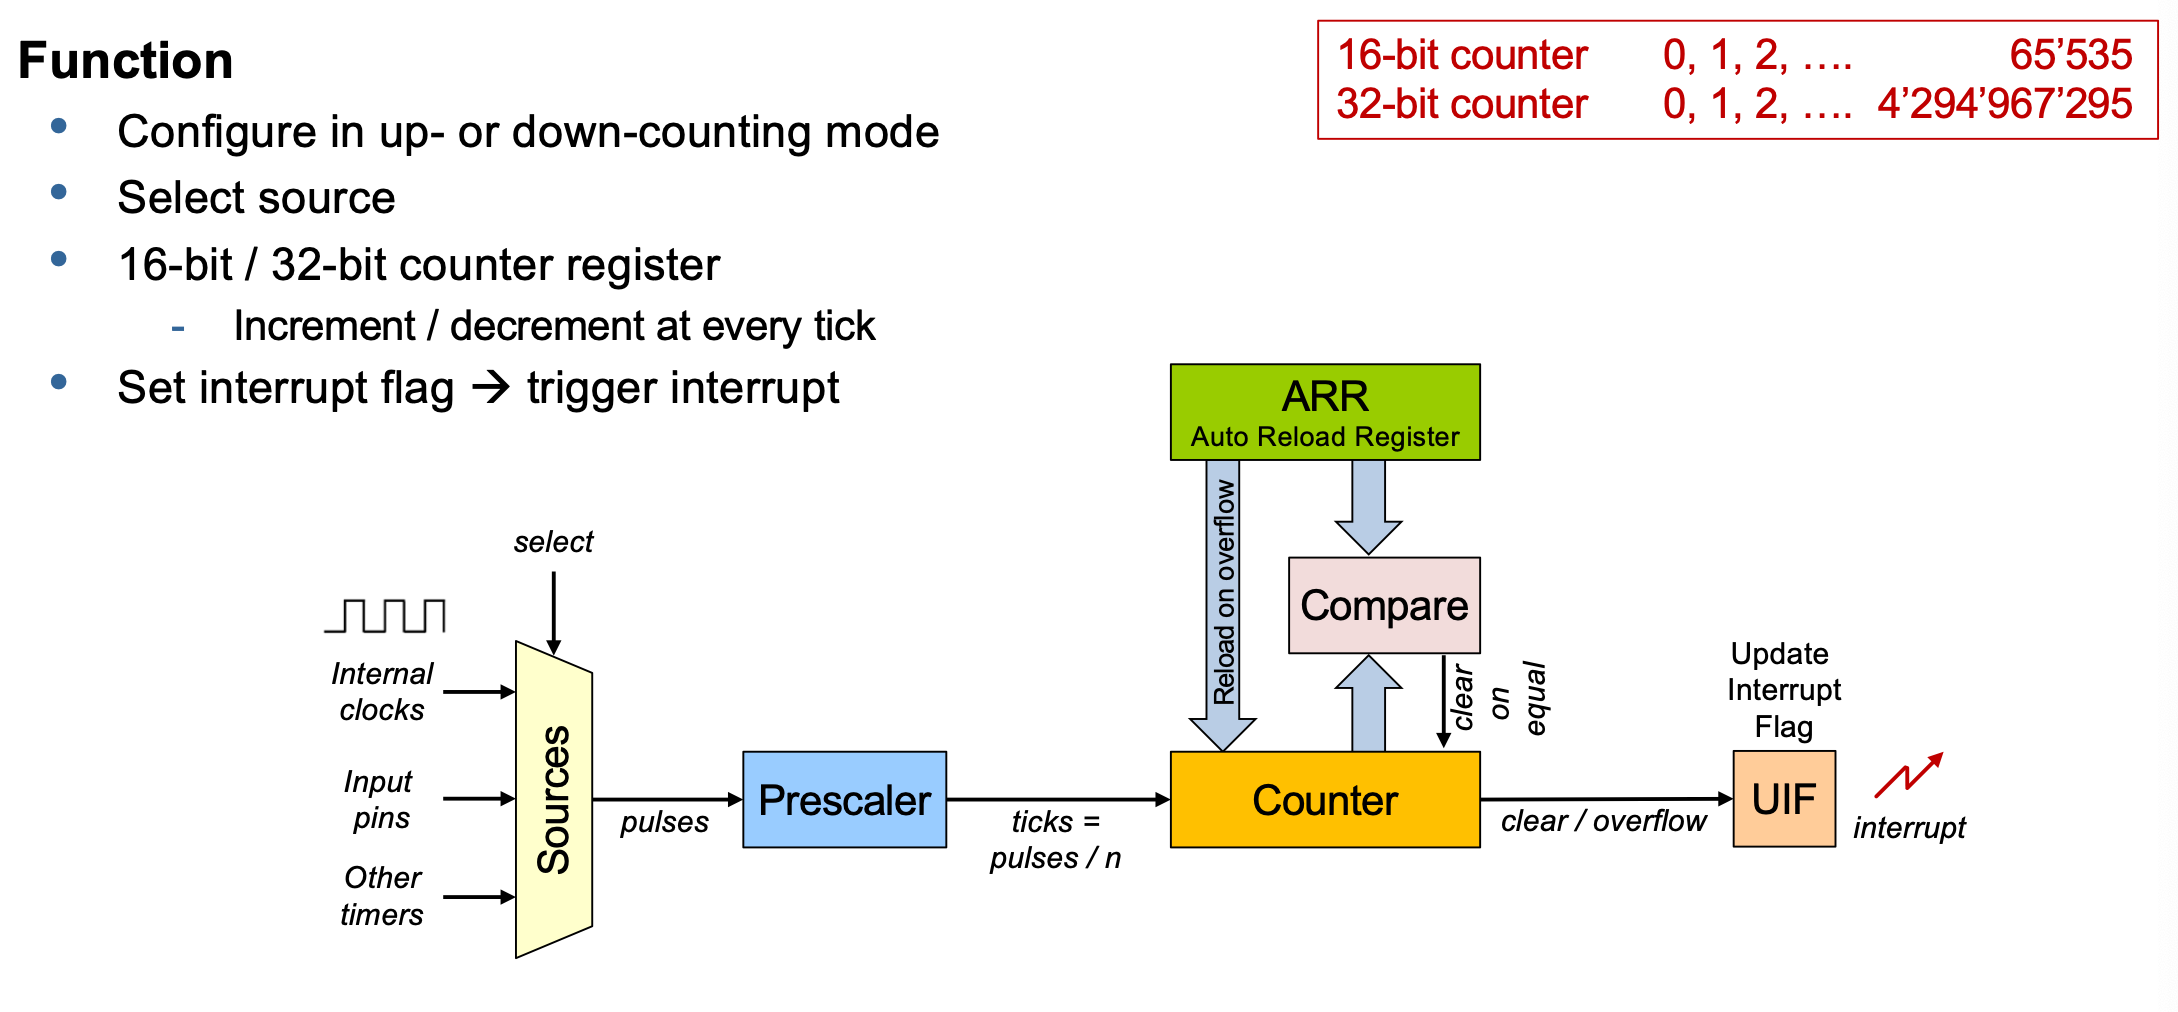
\includegraphics[width=0.3\textwidth]{sections/images/timer_func.png}
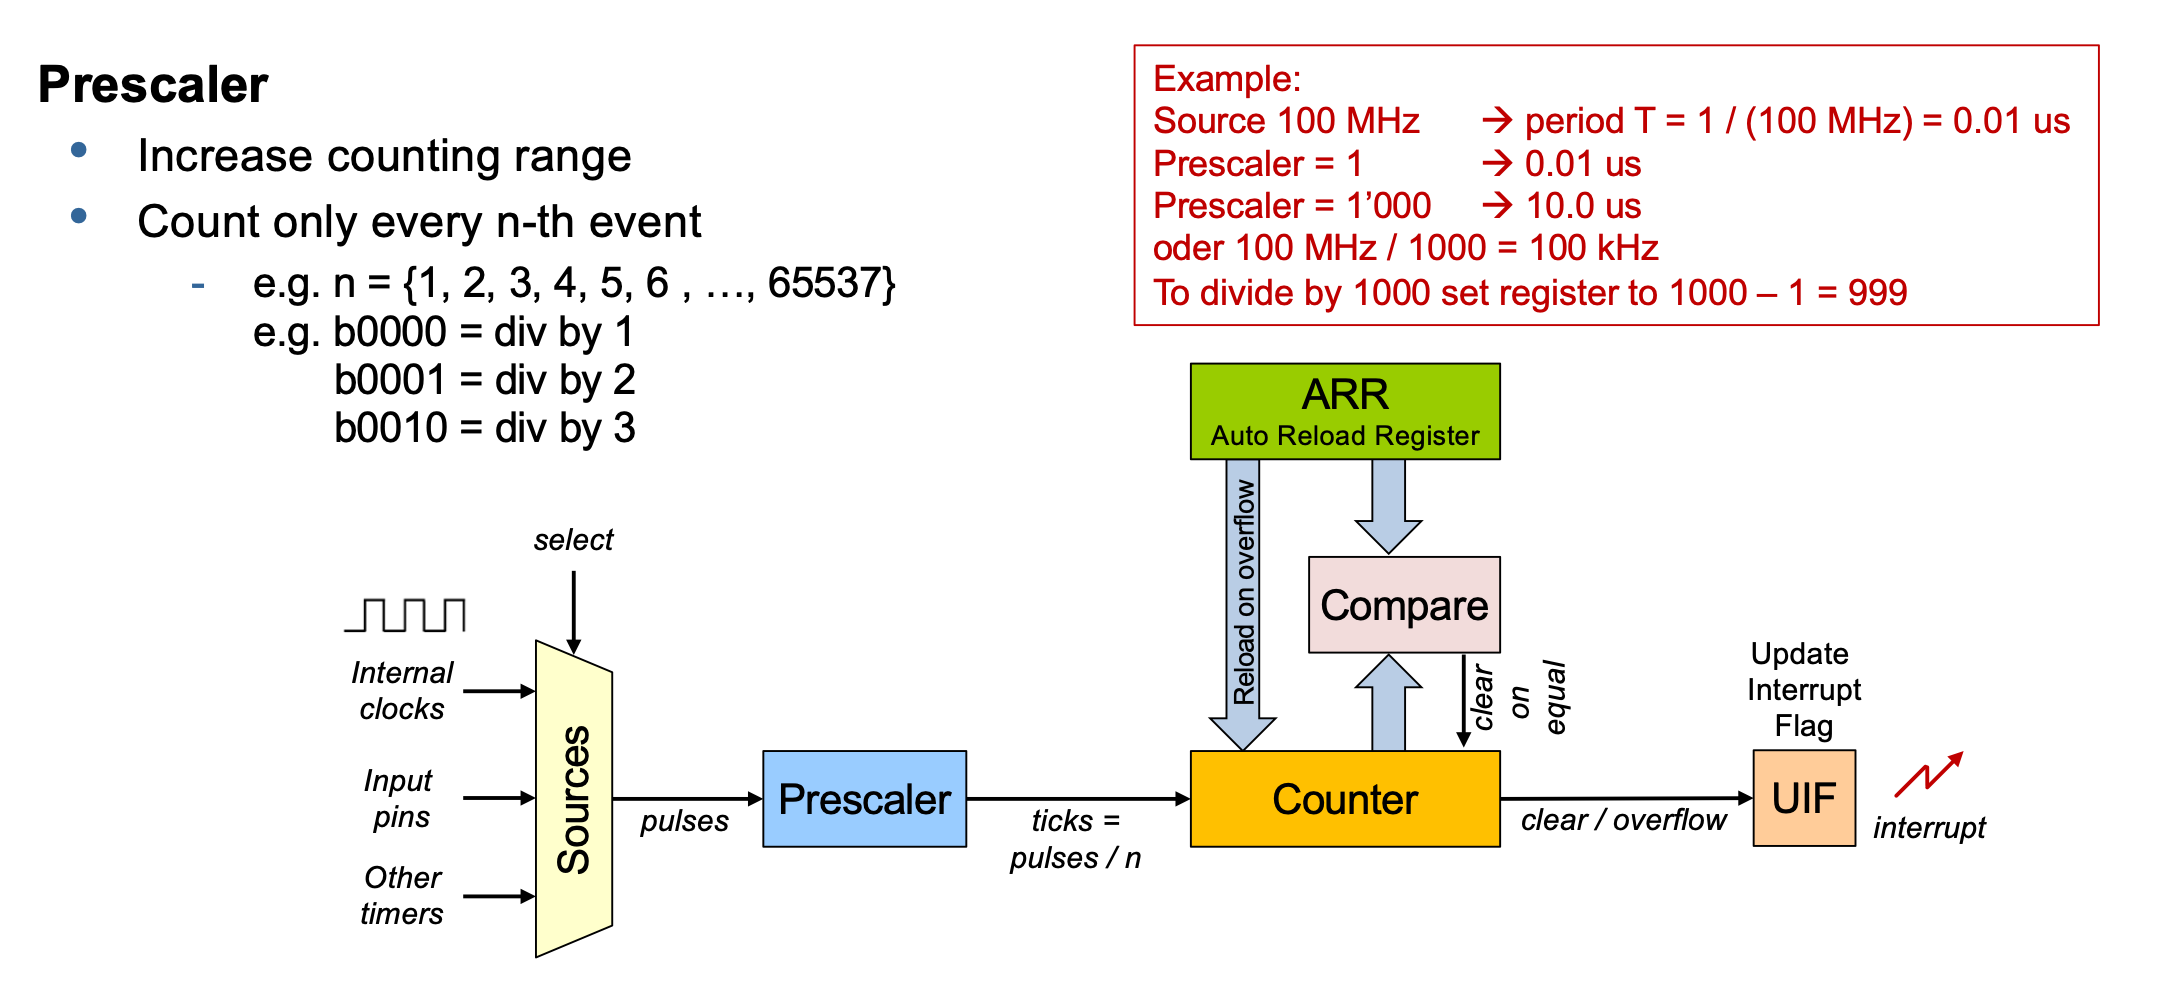
\includegraphics[width=0.3\textwidth]{sections/images/timer_prescaler.png}
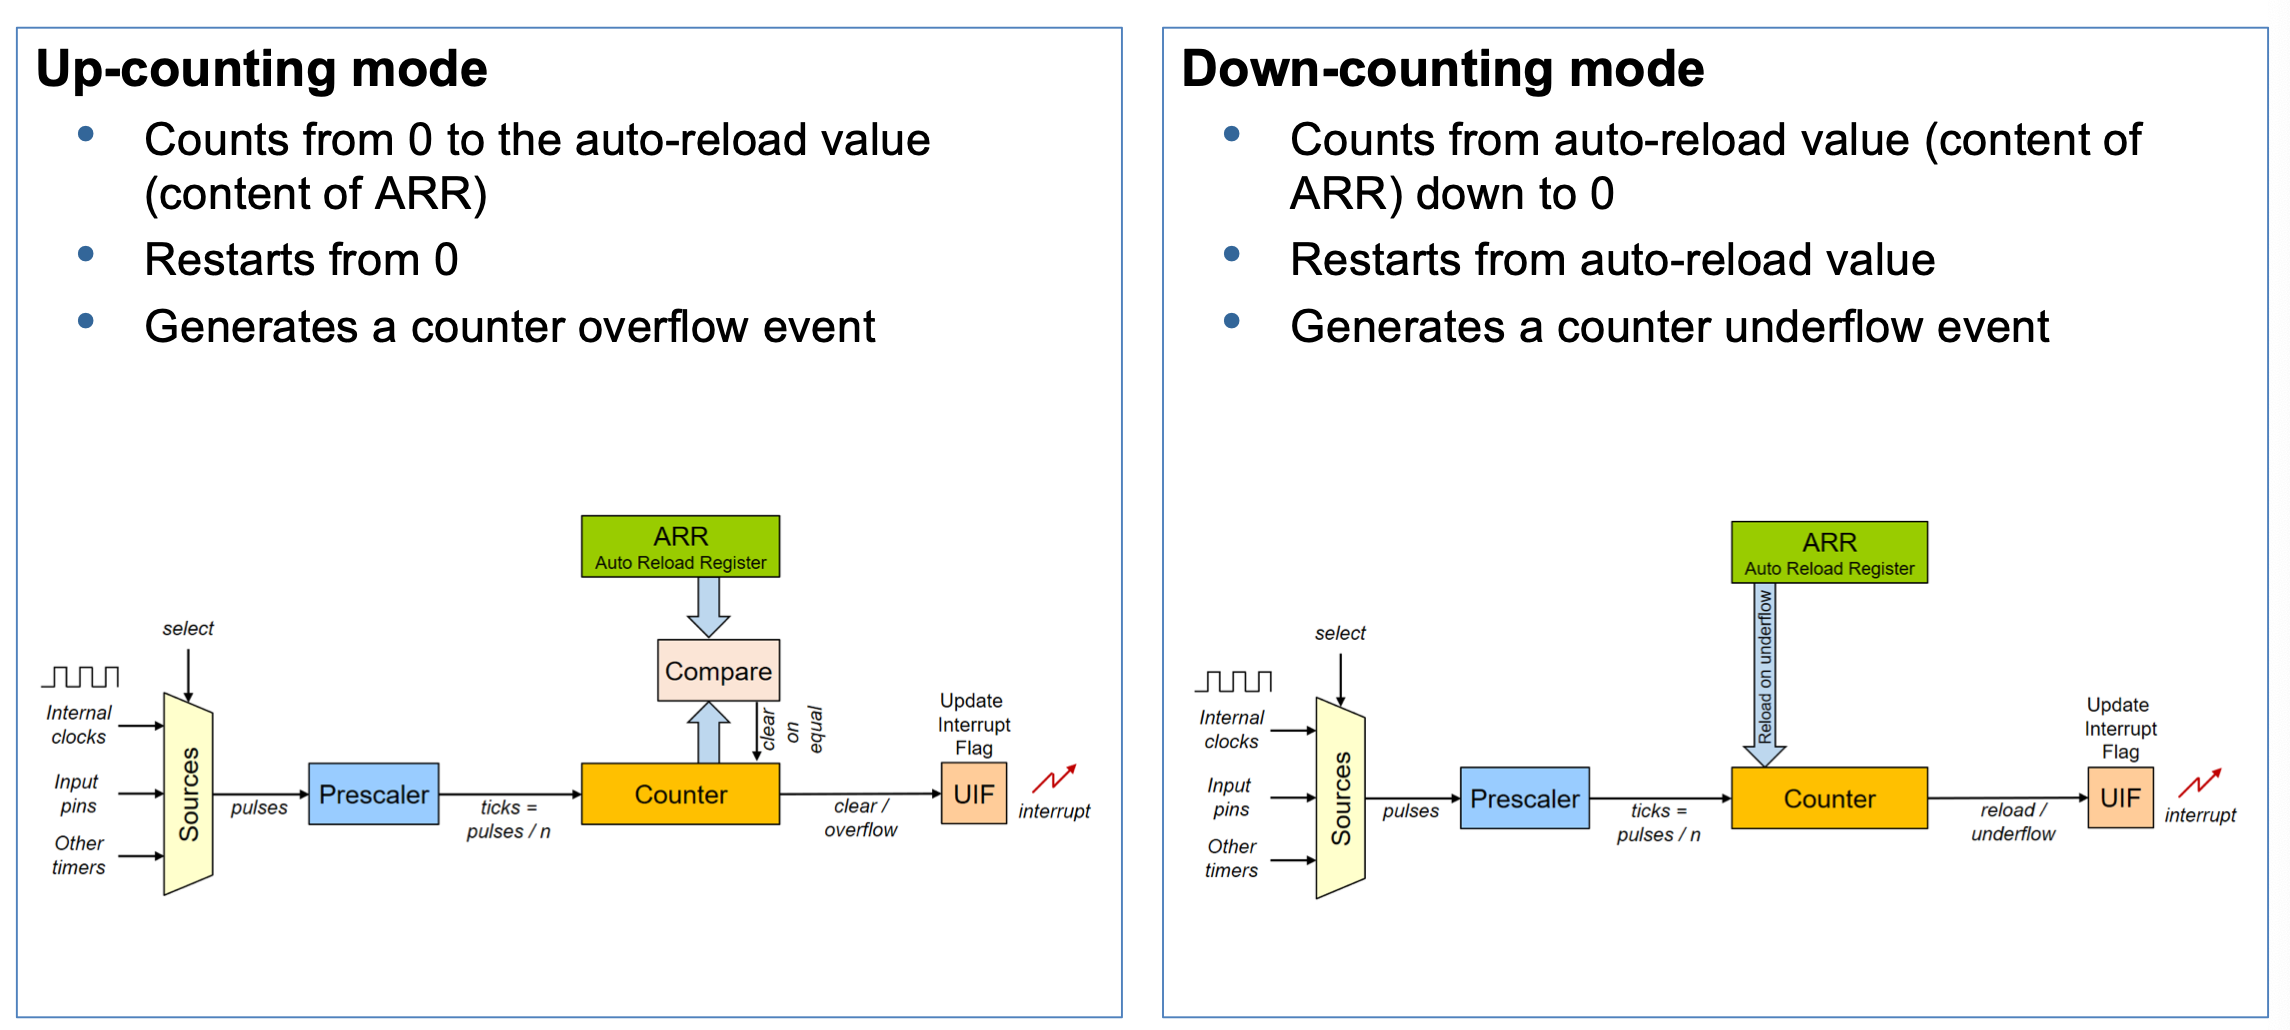
\includegraphics[width=0.3\textwidth]{sections/images/timer_up_down.png}

\subsubsection{Timer Abwärtszählen Beispiel}
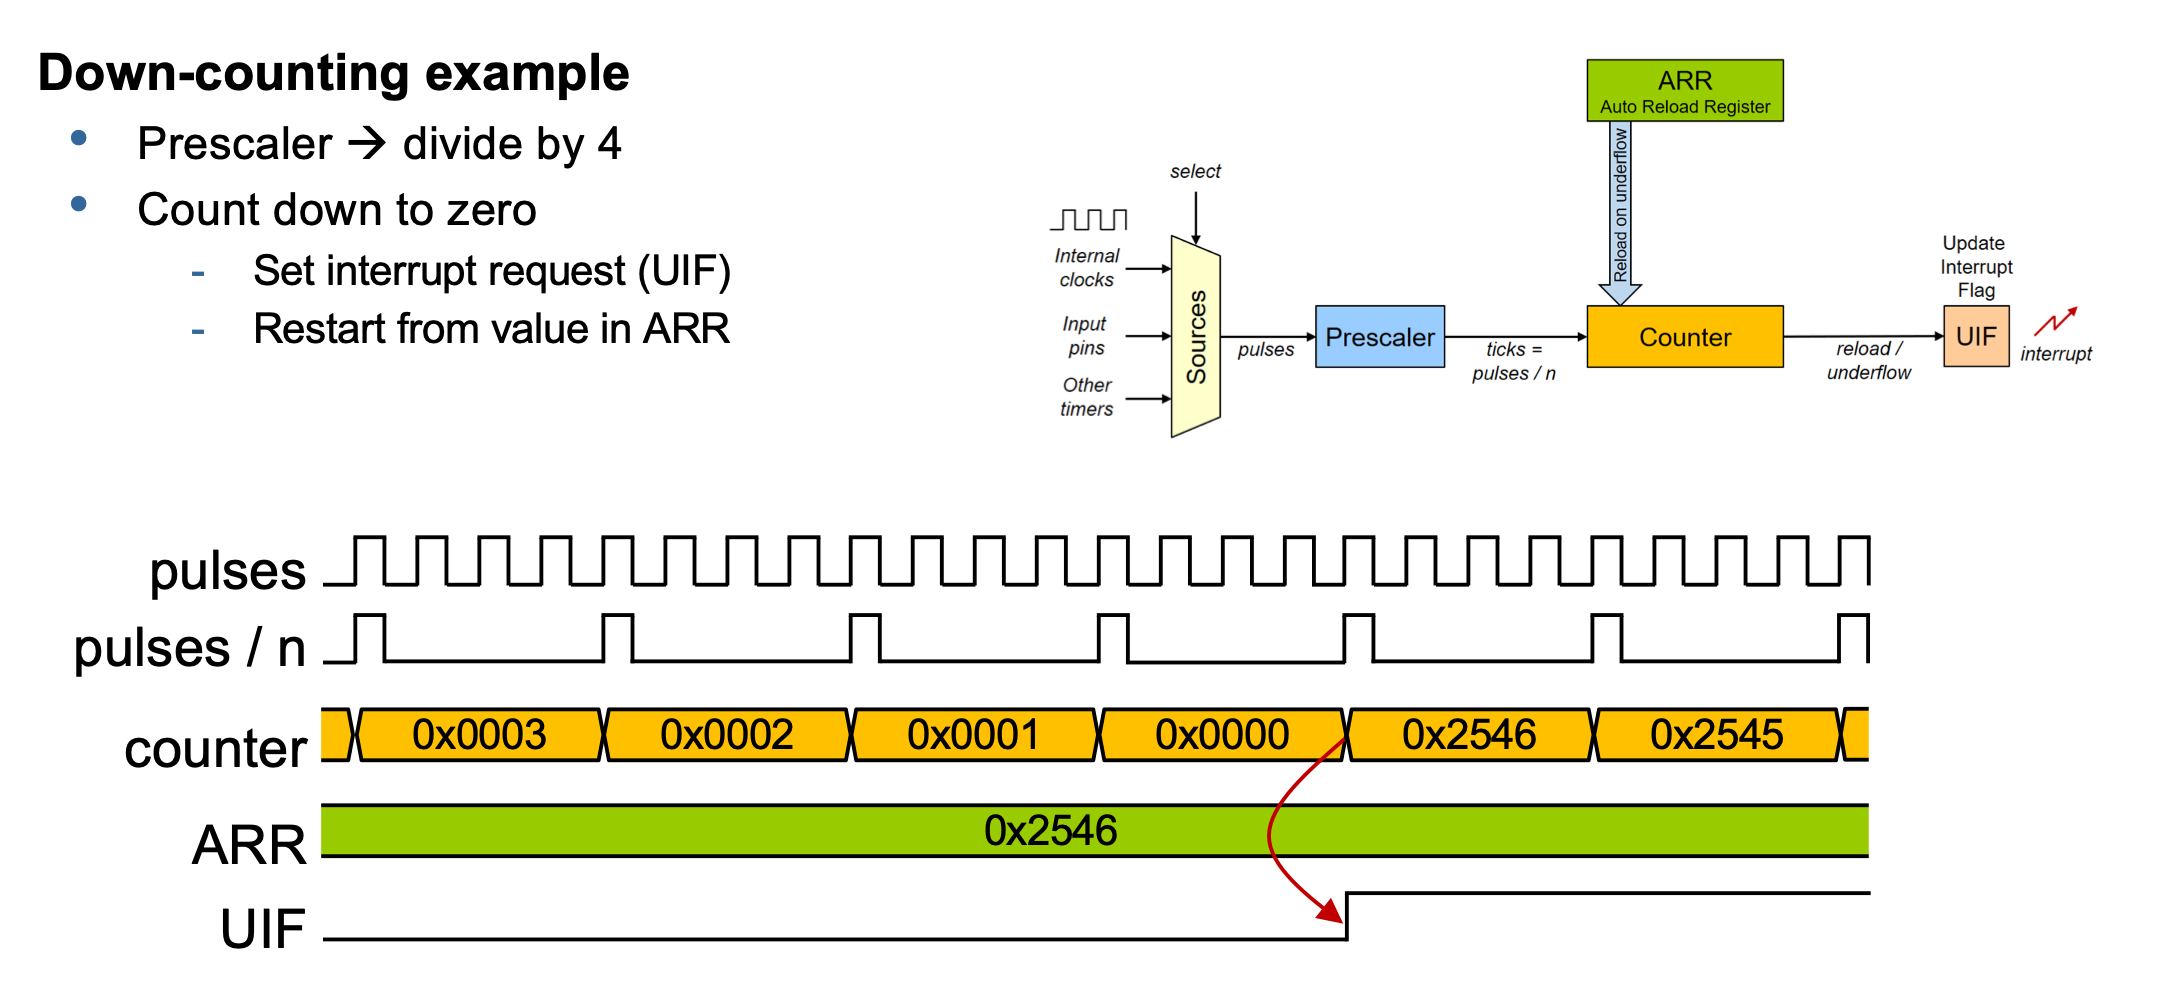
\includegraphics[width=0.3\textwidth]{sections/images/timer_down.png}
\includegraphics[width=0.3\textwidth]{sections/images/timer_down_exp.png}
\includegraphics[width=0.3\textwidth]{sections/images/timer_down2.png}

\subsubsection{Timer Aufwärtszählen Beispiel}
\includegraphics[width=0.3\textwidth]{sections/images/timer_up.png}
\includegraphics[width=0.3\textwidth]{sections/images/timer_up2.png}

\subsubsection{Timer up/down}
\includegraphics[width=0.3\textwidth]{sections/images/timer_up_down2.png}

\subsection{Timer Konfiguration auf STM32}
\begin{itemize}
    \item 16-Bit Timer: TIM3, TIM4
    \item 32-Bit Timer: TIM2, TIM5
\end{itemize}
\includegraphics[width=0.3\textwidth]{sections/images/timer_en.png}
\includegraphics[width=0.3\textwidth]{sections/images/timer_register.png}
\includegraphics[width=0.3\textwidth]{sections/images/timer_register2.png}
\includegraphics[width=0.3\textwidth]{sections/images/timer_config.png}
\includegraphics[width=0.3\textwidth]{sections/images/timer_config2.png}
\includegraphics[width=0.3\textwidth]{sections/images/timer_prescaler_example.png}
\includegraphics[width=0.3\textwidth]{sections/images/timer_config3.png}

\subsection{Timer Beispiel}
\begin{itemize}
    \item Gegeben: CK\_INT = 84 MHz
    \item Interrupt soll alle 1s ausgelöst werden
    \item Timer 3 (16-Bit) verwenden in up-counting Modus
\end{itemize}
\includegraphics[width=0.3\textwidth]{sections/images/timer_ex1.png}
\includegraphics[width=0.3\textwidth]{sections/images/tim_ex2.png}
\includegraphics[width=0.3\textwidth]{sections/images/tim_ex3.png}
\includegraphics[width=0.3\textwidth]{sections/images/tim_ex4.png}

\subsection{Input Capture}
\includegraphics[width=0.3\textwidth]{sections/images/input_capture.png}
\includegraphics[width=0.3\textwidth]{sections/images/input_capture2.png}

\subsection{Pulse Width Modulation (PWM)}
\includegraphics[width=0.3\textwidth]{sections/images/pwm.png}
\includegraphics[width=0.3\textwidth]{sections/images/pwm1.png}
\includegraphics[width=0.3\textwidth]{sections/images/pwm2.png}
\includegraphics[width=0.3\textwidth]{sections/images/pwm3.png}
\includegraphics[width=0.3\textwidth]{sections/images/pwm4.png}

\subsection{PWM output cookbook}
\includegraphics[width=0.3\textwidth]{sections/images/pwm_cookbook.png}
\includegraphics[width=0.3\textwidth]{sections/images/pwm_macros.png}

\subsection{PWM Beispiel}
\includegraphics[width=0.3\textwidth]{sections/images/pwm_exp1.png}
\includegraphics[width=0.3\textwidth]{sections/images/pwm_exp_sol.png}